% !TEX program = pdflatex
% IEEE Conference/Journal Paper - Neuro-Symbolic Fraud Detection

\documentclass[journal]{IEEEtran}

% ============================================================
% Packages
% ============================================================
\usepackage{cite}
\usepackage{amsmath,amssymb,amsfonts}
\usepackage{algorithmic}
\usepackage{algorithm}
\usepackage{graphicx}
\usepackage{textcomp}
\usepackage{xcolor}
\usepackage{booktabs}
\usepackage{multirow}
\usepackage{hyperref}
\usepackage{microtype}
\usepackage[caption=false,font=footnotesize]{subfig}
\usepackage{array}
\usepackage{tabularx}
\usepackage{tikz}
\usetikzlibrary{positioning, arrows.meta, shapes.geometric, backgrounds, shadows}

\hypersetup{
    colorlinks=true,
    linkcolor=blue,
    citecolor=blue,
    urlcolor=blue
}

\def\BibTeX{{\rm B\kern-.05em{\sc i\kern-.025em b}\kern-.08em
    T\kern-.1667em\lower.7ex\hbox{E}\kern-.125emX}}

\begin{document}

% ============================================================
% Title and Authors
% ============================================================
\title{Evidence-Grounded and Cost-Aware Neuro-Symbolic Fraud Investigation with Selective LLM Escalation}

\author{
\IEEEauthorblockN{Harsha Reddy}
\IEEEauthorblockA{
\textit{Independent Researcher} \\
San Francisco, CA, USA \\
harshareddy@example.com}
}

\maketitle

% ============================================================
% Abstract
% ============================================================
\begin{abstract}
Financial institutions face a dual challenge in fraud detection: achieving high recall to reduce the risk of missed suspicious activity, while simultaneously generating compliance-oriented Suspicious Activity Reports (SARs) that require human-readable explanations grounded in verifiable evidence. Existing approaches address these challenges in isolation---tabular models like XGBoost achieve strong detection performance but operate as black boxes, while Large Language Models (LLMs) can generate fluent narratives but are prone to hallucination when untethered from deterministic reasoning. We propose a neuro-symbolic framework that bridges this gap through a four-stage systems architecture. First, an Ensemble Model combines the raw predictive power of XGBoost with the topological explainability of THA-GAT (Temporal-Heterogeneous Attention Graph Network), a task-specific temporal-heterogeneous attention architecture designed specifically to model five heterogeneous entity relationships plus self-loops as an explainability substrate. Second, an attribution pipeline extracts verifiable evidence from THA-GAT via GNNExplainer. Third, a constrained LLM generates SAR narratives grounded in this evidence. Finally, a Neuro-Symbolic Claim Verifier parses LLM-generated SARs and checks all structural claims against the GNN evidence. Evaluated on the IEEE-CIS Fraud Detection dataset (590,540 transactions, 831,392 heterogeneous edges), we demonstrate that while THA-GAT sacrifices raw global ranking performance for topological modeling, the XGBoost-GNN ensemble recovers a 0.8815 AUC. By lowering the escalation threshold to $\theta^* = 0.20$, the ensemble achieves a $95.0\%$ fraud-recall operating point while reducing daily GenAI API expenditure by 44.0\%. Furthermore, our Claim Verifier reduces unsupported structural claims from 26.8\% to 1.0\%, and the online scoring stage achieved a P95 latency of 22.0ms in our benchmark. These results demonstrate a practical pathway toward evidence-grounded and compliance-oriented fraud detection systems.
\end{abstract}

\begin{IEEEkeywords}
Fraud Detection, Graph Neural Networks, Large Language Models, Explainable AI, Neuro-Symbolic AI, Suspicious Activity Reports, Financial Compliance, Temporal Graphs, Graph Attention Networks, Cost Optimization
\end{IEEEkeywords}

% ============================================================
% I. INTRODUCTION
% ============================================================
\section{Introduction}

Financial fraud remains one of the most persistent and economically damaging challenges facing the global financial system. According to the Association of Certified Fraud Examiners, organizations lose an estimated 5\% of their annual revenue to fraud, translating to more than \$5~trillion in global losses annually~\cite{acfe2024}. In the United States alone, the Federal Trade Commission reported over 2.6~million fraud cases in 2023, with losses exceeding \$10~billion~\cite{ftc2024}. The sophistication of modern fraud schemes---including synthetic identity fraud, account takeover rings, and coordinated card-not-present attacks---has outpaced traditional rule-based detection systems, creating an urgent need for advanced machine learning approaches.

Regulatory bodies have responded with increasingly stringent compliance requirements. The U.S.\ Financial Crimes Enforcement Network (FinCEN) mandates that financial institutions file Suspicious Activity Reports (SARs) under the Bank Secrecy Act (BSA) for any transaction that ``the financial institution knows, suspects, or has reason to suspect'' involves funds derived from illegal activity (31~CFR~\S1020.320)~\cite{fincen2020}. Each SAR must contain a detailed narrative explaining the nature of the suspicious activity, the entities involved, and the evidence supporting the suspicion. In 2023, U.S.\ financial institutions filed over 4.6~million SARs, each requiring significant analyst labor to draft.

This regulatory reality creates a dual optimization challenge: financial institutions must simultaneously maximize \emph{detection recall} (reducing the risk of missed suspicious activity) and minimize \emph{investigation cost} (to scale SAR generation across millions of daily transactions). Documented enforcement actions, such as the \$140M USAA penalty~\cite{fincen2022usaa}, illustrate the severe financial significance of compliance failures. Neither objective can be solved independently.

\subsection{The Limitations of Existing Approaches}

Recent advances in Graph Neural Networks (GNNs) have demonstrated significant improvements in fraud detection by modeling transactions as nodes in a graph connected by shared attributes such as payment cards, devices, email addresses, and billing addresses~\cite{zhang2019hetgnn, dou2020care}. By propagating information along these edges through message-passing layers, GNNs can detect coordinated fraud rings that appear innocuous when examined in isolation. However, GNNs suffer from two critical limitations in production deployment:

\textbf{Black-box predictions.} GNNs produce continuous risk scores without human-interpretable explanations. When a GNN flags a transaction with score 0.87, compliance officers cannot determine \emph{why} it was flagged---which relationships contributed, which features were anomalous, or whether the flag reflects genuine suspicion versus a model artifact. FinCEN guidance emphasizes complete descriptions of suspicious activity and relevant supporting information; graph-based entity-link evidence can provide a structured mechanism for representing such relationships. However, tabular models abstract this relational topology away. This opacity can make it difficult to construct complete, evidence-grounded SAR narratives.

\textbf{Temporal na\"{i}vet\'{e}.} Most deployed GNN architectures treat the transaction graph as static, assigning equal weight to a shared-device connection from yesterday and one from six months ago. In reality, the temporal proximity of suspicious connections is a critical signal: a card that shared a device with a confirmed fraudulent card \emph{three days ago} is far more suspicious than one that shared a device \emph{two years ago}.

Concurrently, Large Language Models (LLMs) have shown remarkable capability in generating coherent, context-aware text~\cite{achiam2023gpt4}. Financial institutions have begun experimenting with LLMs for automated SAR narrative generation. However, LLMs deployed without deterministic grounding suffer from a well-documented failure mode: hallucination. An LLM tasked with explaining why a transaction is suspicious may fabricate entity relationships (``this card was linked to a known money laundering network'') or invent risk indicators (``the transaction occurred at 3:47 AM, a known high-risk time'') that have no basis in the actual data~\cite{ji2023hallucination}. In a regulatory context, hallucinated SAR narratives constitute potential filing violations, exposing the institution to both regulatory sanctions and litigation risk.

\textbf{Hybrid systems without cost control} that route every transaction through a generative AI API incur prohibitive operational costs at enterprise scale. For the cost simulation, we assume an effective LLM cost of \$0.012 per invocation based on the model and token-budget configuration used in our experiments. Processing 1~million daily transactions through an LLM at this rate costs approximately \$12,000 per day---\$4.38~million annually---before accounting for engineering overhead~\cite{google_pricing}.

\subsection{Our Approach: Neuro-Symbolic Integration}

We propose a neuro-symbolic framework that addresses all three challenges---detection quality, explainability, and cost efficiency---through a tightly integrated four-stage pipeline:

\begin{enumerate}
    \item \textbf{Stage 1---Detection (Ensemble Model):} Real-time scoring using an ensemble of XGBoost (for tabular anomaly detection) and THA-GAT (a Temporal-Heterogeneous Attention Graph Network). While THA-GAT trades off raw AUC for multi-modal structural priors, it serves as the critical \emph{explainability substrate}.
    \item \textbf{Stage 2---Attribution (GNNExplainer):} For transactions exceeding a learned cost-optimized escalation threshold, we extract model-attributed evidence, identifying exactly which features and graph relationships (e.g. shared devices) drove the prediction.
    \item \textbf{Stage 3---Generation (Constrained LLM):} The attribution vector is serialized into a structured prompt that constrains a Large Language Model to generate SAR narratives.
    \item \textbf{Stage 4---Verification (Claim Verifier):} A post-processing symbolic layer extracts model-attributed evidence and verifies the factual existence of the corresponding graph relationships claimed by the LLM, reducing unsupported claims.
\end{enumerate}

\subsection{Contributions}

The key contributions of this paper are:

\begin{enumerate}
\item \textbf{THA-GAT Architecture} (Section~\ref{sec:thagat}): A heterogeneous graph attention network with per-edge-type query/key/value projections, learnable temporal decay attention, LayerNorm with residual connections, and a fraud-ring-aware subgraph readout mechanism that combines node-level and neighborhood-level scoring through a learned sigmoid gate. With 3,367,166 trainable parameters, it serves as the relational substrate.

\item \textbf{Attribution-Grounded SAR Generation} (Section~\ref{sec:attribution}): A two-stage pipeline that uses Integrated Gradients and edge-masking attribution from GNNExplainer to constrain LLM-generated SAR drafts, reducing unsupported claims by requiring supported structural assertions to map to a verified feature or edge attribution. To our knowledge, we did not identify prior fraud-detection studies that evaluated GNNExplainer-derived evidence as a structured constraint for LLM-based SAR drafting.

\item \textbf{Cost-Optimized Escalation Framework} (Section~\ref{sec:cost}): A formal constrained optimization that sweeps the escalation threshold $\theta$ to find the cost-minimizing operating point under the recall constraint, reducing daily costs by 44.0\% (\$5,281/day savings, \$1.93M/year) while maintaining 95.0\% recall.

\item \textbf{Pipeline Stage Architecture} (Section~\ref{sec:architecture}): A deployment-oriented pipeline using Apache Kafka for transaction ingestion, Redis for real-time feature store and neighborhood caching, and a FastAPI serving layer that orchestrates the detection-attribution-compliance pipeline with sub-second latency targets.

\item \textbf{Ablation Analysis} (Section~\ref{sec:ablation}): Comparative architectural ablation study evaluating the effect of temporal, heterogeneous, and graph-structural design choices on detection performance.
\end{enumerate}

The remainder of this paper is organized as follows: Section~II surveys related work across graph-based fraud detection, LLMs for financial compliance, and explainable AI. Section~III details the methodology including graph construction, the THA-GAT architecture, the attribution pipeline, the cost-optimization framework, and the streaming deployment architecture. Section~IV describes the experimental setup. Section~V presents results including detection performance, cost analysis, ablation studies, and qualitative SAR examples. Section~VI discusses implications and limitations. Section~VII concludes.

% ============================================================
% II. RELATED WORK
% ============================================================
\section{Related Work}

\subsection{Graph Neural Networks for Fraud Detection}

The application of graph neural networks to fraud detection has grown rapidly since the seminal work of Kipf and Welling~\cite{kipf2017gcn} on Graph Convolutional Networks (GCN). Early applications modeled user-item interactions as bipartite graphs and applied spectral convolutions to detect anomalous purchasing patterns~\cite{hamilton2017rep}.

\textbf{Homogeneous approaches.} GeniePath~\cite{liu2019geniepath} introduced adaptive path aggregation for fraud detection on Alipay's transaction graph, demonstrating that learned aggregation strategies outperform fixed-depth message passing. GraphSAGE~\cite{hamilton2017graphsage} enabled inductive learning on unseen nodes, a critical requirement for fraud systems where new transactions arrive continuously. However, these homogeneous approaches treat all edges identically, losing the rich semantic information encoded in different relationship types.

\textbf{Heterogeneous approaches.} The recognition that fraud graphs are inherently multi-relational motivated heterogeneous graph architectures. HetGNN~\cite{zhang2019hetgnn} and HAN~\cite{wang2019han} demonstrated that encoding multiple node and edge types improves detection of complex fraud rings by allowing the model to learn distinct aggregation patterns for different relationship semantics. CARE-GNN~\cite{dou2020care} specifically addressed the camouflage problem where fraudsters deliberately forge connections with legitimate users to blend in, proposing a reinforcement-learning-based neighbor selector that filters suspicious edges. PC-GNN~\cite{liu2021pcgnn} partitioned the graph by label to mitigate the imbalance problem inherent in fraud detection.

\textbf{Temporal approaches.} Static graph models ignore a crucial dimension of fraud detection: time. TGN~\cite{rossi2020tgn} introduced dynamic graph modeling that captures evolving user behavior using memory modules. TGAT~\cite{xu2020tgat} applied time-decaying attention weights to temporal graphs, demonstrating that temporal encoding effectively models the diminishing relevance of old connections. EvolveGCN~\cite{pareja2020evolvegcn} proposed adapting GCN weights over time to capture continuous-time dynamics for temporal graph learning.

Our THA-GAT differs from these approaches in three ways: (1) we parameterize the temporal decay rate $\lambda_r$ independently for each edge type, allowing the model to learn that device-sharing connections decay faster than card co-occurrence patterns; (2) we introduce a fraud-ring-aware subgraph readout that jointly scores node-level and neighborhood-level suspicion through degree statistics and pooled embeddings; and (3) we design the architecture specifically for downstream explainability, ensuring that attention weights and temporal decay factors are inspectable.

\subsection{Explainable AI for Graph Neural Networks}

Post-hoc explainability for GNNs has been an active research area. GNNExplainer~\cite{ying2019gnnexplainer} identifies the minimal subgraph and feature subset that preserve a model's prediction by learning soft edge and feature masks. PGExplainer~\cite{luo2020pgexplainer} scales this approach to the inductive setting by learning a global edge-mask generator. SubgraphX~\cite{yuan2021subgraphx} uses Monte Carlo Tree Search to find explanatory subgraphs. More recently, CF-GNNExplainer~\cite{lucic2022cfgnn} generates counterfactual explanations (``what would need to change to flip the prediction?'').

While these tools have been applied to fraud detection for debugging and model validation~\cite{tang2024explainable}, we did not identify prior studies that leveraged their output as a structured input to downstream generation systems. We propose a novel use: feeding GNNExplainer attributions as constraints into an LLM prompt, creating what we term ``attribution-grounded'' natural language generation. This bridges the gap between post-hoc explanation and actionable compliance output.

\subsection{LLMs for Financial Compliance and Fraud}

The application of LLMs to financial compliance is nascent but growing rapidly. FinGPT~\cite{yang2023fingpt} fine-tuned open-source LLMs on financial data for sentiment analysis and risk assessment, proving that localized models can achieve strong performance in highly specialized domains. Similarly, BloombergGPT~\cite{wu2023bloomberggpt} demonstrated that domain-specific pre-training on large-scale financial text corpus improves performance on financial NLP tasks significantly over general-purpose models. 

However, deploying generative models in highly regulated sectors like banking is constrained by the persistent issue of hallucination~\cite{ji2023hallucination}. In the specific context of fraud detection and Suspicious Activity Reports, producing a false claim about a customer's transaction history can lead to severe legal and reputational damage. Recent paradigms have explored integrating GNNs with LLMs for financial crime investigation, including multimodal graph-LLM frameworks for illicit-activity narratives~\cite{multimodal2023}, GraphLIME-based explanation pipelines for anomaly detection~\cite{graphlime2023}, and $k$-hop subgraph-to-LLM reasoning systems~\cite{khop2023}. However, these approaches often pass raw subgraphs or post-hoc node explanations to generative models without strict topological constraint enforcement. We did not identify prior fraud-detection frameworks that explicitly use edge-type-specific temporal attention weights as a deterministically verified constraint for downstream SAR generation.

In generative approaches without explicit model attribution, the LLM receives historical neighborhood context but not the specific attention weights and feature importances that drove the algorithmic prediction. Without strict deterministic grounding, the model risks narrative hallucination---inventing plausible but factually incorrect relationships between entities to justify its output.

Our attribution-grounded approach provides a traceable chain of evidence, generating compliance-oriented narratives (SARs) that support formatting requirements with reduced risk of unsupported claims.

\subsection{Edge-Aware and Attention-Based Graph Models}

Several recent works have explored edge-type-specific attention mechanisms. The original Heterogeneous Graph Attention Network (HAN)~\cite{wang2019han} proposed node-level and semantic-level attention but lacked temporal decay. Edge-aware attention has also been explored in broader domains, such as molecular property prediction~\cite{yang2019analyzing}, where edge features explicitly modulate message passing.

Our THA-GAT synthesizes insights from these works---per-edge-type projections from heterogeneous graph networks, temporal decay from continuous-time temporal graphs, and subgraph-level readout logic---but uniquely combines all three within a single architecture explicitly designed for the specific downstream requirements of regulatory compliance automation.

\subsection{Cost-Aware Machine Learning Deployment}

The economics of AI deployment have received increasing attention. Cascade architectures~\cite{wang2023wisdom} route easy examples through cheap models and hard examples through expensive ones. FrugalGPT~\cite{chen2023frugalgpt} demonstrated significant cost reductions by learning to select among LLMs of different price points. However, to our knowledge, no prior work has formalized the cost-recall tradeoff specifically for the GNN-to-LLM escalation in fraud detection, nor provided the cost-recall trade-off analysis we present in Section~\ref{sec:cost}.

% ============================================================
% III. METHODOLOGY
% ============================================================
\section{Methodology}

\subsection{System Overview}

Fig.~\ref{fig:system} illustrates the complete neuro-symbolic pipeline. The system operates in two phases:

\textbf{Training Phase:} Raw transaction data undergoes chronological splitting (70\% Train, 15\% Validation, 15\% Test). The training set is used to fit the models. The validation set is exclusively used to optimize the cost-recall escalation threshold ($\theta^*$). The final ensemble uses a fixed equal weighting of the two model probabilities. All final reported metrics in Section~\ref{sec:results} are evaluated on the untouched out-of-time Test set to prevent data leakage (though Test transactions can form edges to historical nodes in the training/validation periods to maintain temporal continuity). Feature engineering yields 32 curated features, and heterogeneous graph construction yields 6 edge types. THA-GAT is trained on the graph using BCEWithLogitsLoss with class-imbalance weighting. Post-training, the GNNExplainer-based attribution module is applied to escalated transactions.

\textbf{Inference Phase:} Incoming transactions are ingested via Apache Kafka, enriched with real-time features from Redis, and scored by the trained models. The final risk score used for escalation is computed via an unweighted ensemble:
\begin{equation}
S_{ensemble} = 0.5 \cdot S_{XGB} + 0.5 \cdot S_{THA-GAT}
\end{equation}
where $S_{XGB}$ and $S_{THA-GAT}$ are the model risk scores of XGBoost and THA-GAT. Equal weighting was selected as a fixed, non-optimized ensemble rule to avoid introducing an additional validation-tuned parameter. Transactions where $S_{ensemble} \ge \theta^*$ undergo GNNExplainer attribution followed by constrained LLM SAR generation via Google Gemini.

\begin{figure}[!t]
\centering
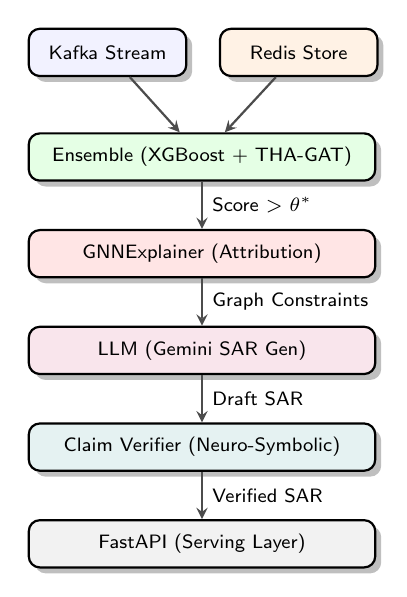
\begin{tikzpicture}[
    >=stealth,
    node distance=0.6cm and 0.4cm,
    font=\sffamily\scriptsize,
    box/.style={draw, rectangle, rounded corners, minimum width=2cm, minimum height=0.6cm, align=center, fill=blue!5, drop shadow, thick},
    arrow/.style={->, thick, draw=black!70}
]
% Nodes
\node[box] (kafka) {Kafka Stream};
\node[box, right=of kafka, fill=orange!10] (redis) {Redis Store};
\node[box, below=0.7cm of kafka, xshift=1.2cm, fill=green!10, minimum width=4.4cm] (gnn) {Ensemble (XGBoost + THA-GAT)};
\node[box, below=0.6cm of gnn, fill=red!10, minimum width=4.4cm] (explainer) {GNNExplainer (Attribution)};
\node[box, below=0.6cm of explainer, fill=purple!10, minimum width=4.4cm] (llm) {LLM (Gemini SAR Gen)};
\node[box, below=0.6cm of llm, fill=teal!10, minimum width=4.4cm] (verifier) {Claim Verifier (Neuro-Symbolic)};
\node[box, below=0.6cm of verifier, fill=gray!10, minimum width=4.4cm] (api) {FastAPI (Serving Layer)};

% Edges
\draw[arrow] (kafka) -- (gnn);
\draw[arrow] (redis) -- (gnn);
\draw[arrow] (gnn) -- (explainer) node[midway, right] {Score $>\theta^*$};
\draw[arrow] (explainer) -- (llm) node[midway, right] {Graph Constraints};
\draw[arrow] (llm) -- (verifier) node[midway, right] {Draft SAR};
\draw[arrow] (verifier) -- (api) node[midway, right] {Verified SAR};
\end{tikzpicture}
\caption{End-to-end neuro-symbolic fraud detection pipeline. Stage~1: Ensemble Model (XGBoost + THA-GAT) scores transactions. Stage~2: GNNExplainer extracts feature and edge attributions. Stage~3: Constrained LLM generates attribution-grounded SAR narratives. Stage~4: Neuro-Symbolic Claim Verifier ensures structural claims match attributions. The cost-optimized escalation threshold $\theta^*$ determines which transactions are routed to the LLM.}
\label{fig:system}
\end{figure}

\subsection{Graph Construction}

We construct a heterogeneous transaction graph $\mathcal{G} = (\mathcal{V}, \mathcal{E}, \mathcal{R}, \mathcal{T})$ from the IEEE-CIS Fraud Detection dataset~\cite{ieee_cis}, which contains 590,540 e-commerce transactions released by Vesta Corporation.

\subsubsection{Feature Engineering}

Each transaction node is characterized by 32 carefully curated features spanning six categories:

\textbf{Transaction Metadata (4 features):} TransactionAmt (log-transformed via log1p), TransactionDT (normalized temporal offset), ProductCD (encoded product category), dist1 (geographic distance indicator).

\textbf{Card Attributes (6 features):} card1 through card6, representing card identifier components, card type, and issuing bank information. These serve dual roles as features and as keys for edge construction.

\textbf{Velocity Counters (7 features):} C1, C2, C5, C6, C11, C13, C14---Vesta's proprietary counting features representing the number of transactions sharing specific attributes within rolling time windows. These capture the temporal density of activity.

\textbf{Recency Indicators (5 features):} D1, D2, D4, D10, D15---time deltas between the current transaction and previous transactions associated with the same entity, measuring how recently this payment instrument was active.

\textbf{Behavioral Features (4 features):} V127, V130, V307, V310---selected from Vesta's anonymous feature bank (originally 339 V-features), chosen via correlation analysis for their independent predictive power. Feature selection was performed using training data only to strictly prevent data leakage.

\textbf{Identity Features (6 features):} addr1, addr2 (billing address components), P\_emaildomain, R\_emaildomain (purchaser and recipient email domains), DeviceType, DeviceInfo---linking transactions to physical devices and digital identities.

All numeric features are z-score normalized using training set statistics. Categorical features are label-encoded (with the encoder fit strictly on the training split to prevent data leakage), with missing values imputed as 'unknown' for string columns and 0.0 for numeric columns. 

\subsubsection{Heterogeneous Edge Construction}

We define five semantically distinct co-occurrence relationships, plus self-loops:

\textbf{Card co-occurrence edges ($r_{\text{card}}$):} Two transactions sharing the same (card1, card2) tuple are connected by a card edge, representing usage of the same physical payment instrument. To prevent graph explosion from anomalous high-frequency cards, we restrict to groups of size $1 < n < 60$. For each valid group, we create edges between the first $\min(n, 12)$ temporally ordered transactions with a sliding window of 5, yielding 143,527 edge pairs. 

\textbf{Device co-occurrence edges ($r_{\text{device}}$):} Transactions sharing the same DeviceInfo value (excluding 'unknown') are connected, representing usage of the same physical or virtual device. Window size 4, yielding 10,902 edge pairs. Device co-occurrence is used as a relational signal because legitimate users rarely share devices with strangers.

\textbf{Email domain co-occurrence edges ($r_{\text{email}}$):} Transactions sharing P\_emaildomain or R\_emaildomain are connected. Groups limited to $n < 100$ with window size 3, yielding 378 edge pairs (99 for purchaser domain, 279 for recipient domain).

\textbf{Address co-occurrence edges ($r_{\text{address}}$):} Transactions sharing addr1 or addr2 values, with $n < 80$ and window size 3, yielding 998 edge pairs (727 for addr1, 271 for addr2).

\textbf{Shared-device cross-card edges ($r_{\text{shared\_device}}$):} Shared-device cross-card edges are designed to capture suspicious multi-entity behavior. For each device, we identify transactions from \emph{different} cards that used the same device and connect representative transactions from each card group. This yields 53,202 edge pairs. This edge type is specifically designed to detect account takeover and synthetic identity fraud patterns.

\textbf{Self-loop edges ($r_{\text{self}}$):} Every node receives a self-loop edge, ensuring that isolated nodes still receive a valid embedding update during message passing.

To strictly prevent temporal leakage, the graph is constructed exclusively on the chronological training split (70\% of the 590,540 dataset). This final training graph contains 413,378 nodes and 831,392 total directed edges across 6 relation types (209,007 non-self edge pairs, 418,014 directed non-self edges, and 413,378 self-loop edges). The temporal gap $\Delta t_{ij}$ for each edge is computed as $|\text{TransactionDT}_i - \text{TransactionDT}_j|$ and normalized to zero mean and unit variance across the training set. For each validation/test transaction, graph neighbors were restricted to transactions with timestamps strictly earlier than the target transaction; no future validation/test nodes or labels were used.

\begin{algorithm}[!t]
\caption{Heterogeneous Graph Construction}
\label{alg:graph}
\begin{algorithmic}[1]
\REQUIRE Transaction DataFrame $\mathcal{D}$ with $N$ rows
\ENSURE \texttt{edge\_index}, \texttt{edge\_type}, \texttt{edge\_time\_delta}
\STATE Initialize edges, types, deltas as empty lists
\FOR{each unique (card1, card2) group $G$}
    \IF{$1 < |G| < 60$}
        \FOR{$i = 0$ \TO $\min(|G|-1, 11)$}
            \FOR{$j = i+1$ \TO $\min(|G|-1, i+5)$}
                \STATE Add bidirectional edge $(G[i], G[j])$ 
                \STATE Type = CARD
                \STATE $\Delta t = |DT[G[i]] - DT[G[j]]|$
            \ENDFOR
        \ENDFOR
    \ENDIF
\ENDFOR
\STATE \emph{// Similar loops for Device, Email, Address edges}
\FOR{each unique DeviceInfo $d$}
    \STATE $C \gets \text{group transactions by card within } d$
    \IF{$|C| > 1$}
        \FOR{each pair of card groups $(c_i, c_j)$}
            \STATE Add edge between representative transactions
        \ENDFOR
    \ENDIF
\ENDFOR
\FOR{$i = 1$ \TO $N$}
    \STATE Add self-loop edge $(i, i)$ with type SELF, $\Delta t = 0$
\ENDFOR
\RETURN \texttt{edge\_index}, \texttt{edge\_type}, \texttt{edge\_time\_delta}
\end{algorithmic}
\end{algorithm}

\subsection{THA-GAT Architecture}
\label{sec:thagat}

Fig.~\ref{fig:thagat} shows the THA-GAT architecture consisting of three stacked Temporal-Heterogeneous Attention Layers followed by a Fraud-Ring-Aware Subgraph Readout. The total parameter count is 3,367,166.

\begin{figure}[!t]
\centering
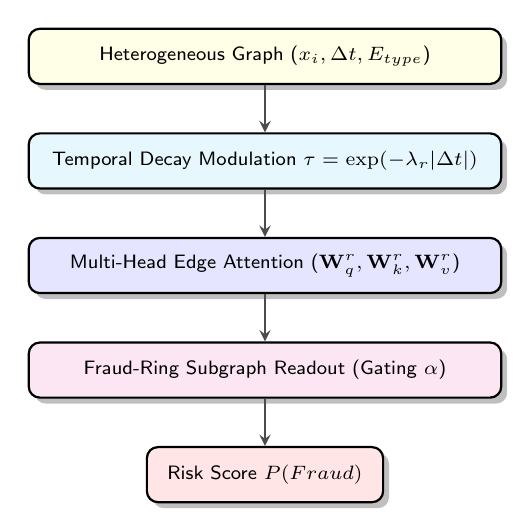
\begin{tikzpicture}[
    >=stealth,
    node distance=0.6cm,
    font=\sffamily\scriptsize,
    box/.style={draw, rectangle, rounded corners, minimum width=6cm, minimum height=0.7cm, align=center, fill=green!5, drop shadow, thick},
    arrow/.style={->, thick, draw=black!70}
]
% Nodes
\node[box, fill=yellow!10] (input) {Heterogeneous Graph ($x_i, \Delta t, E_{type}$)};
\node[box, below=of input, fill=cyan!10] (decay) {Temporal Decay Modulation $\tau = \exp(-\lambda_r |\Delta t|)$};
\node[box, below=of decay, fill=blue!10] (gat) {Multi-Head Edge Attention ($\mathbf{W}_q^r, \mathbf{W}_k^r, \mathbf{W}_v^r$)};
\node[box, below=of gat, fill=magenta!10] (readout) {Fraud-Ring Subgraph Readout (Gating $\alpha$)};
\node[box, below=of readout, fill=red!10, minimum width=3cm] (output) {Risk Score $P(Fraud)$};

% Edges
\draw[arrow] (input) -- (decay);
\draw[arrow] (decay) -- (gat);
\draw[arrow] (gat) -- (readout);
\draw[arrow] (readout) -- (output);
\end{tikzpicture}
\caption{THA-GAT architecture. Three temporal-heterogeneous attention layers with per-edge-type projections ($\mathbf{W}_q^r, \mathbf{W}_k^r, \mathbf{W}_v^r$) and temporal decay modulation $\tau(\Delta t)$. The fraud-ring readout combines node-level and ring-level scores through a learned gate~$\alpha$.}
\label{fig:thagat}
\end{figure}

\subsubsection{Temporal-Heterogeneous Attention Layer}

Each attention layer performs edge-type-conditioned message passing with temporal decay modulation. For each edge type $r \in \mathcal{R} = \{0, 1, \dots, 5\}$, we maintain separate query, key, and value projection matrices:
\begin{equation}
\mathbf{W}_q^r, \mathbf{W}_k^r, \mathbf{W}_v^r \in \mathbb{R}^{d_{\text{in}} \times Hd_h}
\end{equation}
where $H = 4$ is the number of attention heads and $d_h = d_{\text{out}} / H$ is the per-head dimension. This yields $6 \times 3 = 18$ separate linear projections per layer.

For an edge $(i, j)$ of type $r$ with temporal gap $\Delta t_{ij}$, the multi-head attention is computed as:

\textbf{Step 1 --- Type-Conditioned Projection:}
\begin{equation}
\mathbf{q}_i^r = \mathbf{W}_q^r \mathbf{h}_i, \quad \mathbf{k}_j^r = \mathbf{W}_k^r \mathbf{h}_j, \quad \mathbf{v}_j^r = \mathbf{W}_v^r \mathbf{h}_j
\end{equation}

\textbf{Step 2 --- Temporal Decay Modulation:}
\begin{equation}
\tau(\Delta t_{ij}, r) = \exp(-|\lambda_r| \cdot |\Delta t_{ij}|)
\end{equation}
where $\lambda_r \in \mathbb{R}$ is a learnable, per-edge-type decay parameter initialized at 0.01. The absolute value ensures non-negative decay. 

\textbf{Step 3 --- Scaled Dot-Product Attention:}
\begin{equation}
\alpha_{ij}^r = \text{softmax}_j \left( \frac{(\mathbf{q}_i^r)^\top \mathbf{k}_j^r}{\sqrt{d_h}} \cdot \tau(\Delta t_{ij}, r) \right)
\end{equation}

\textbf{Step 4 --- Weighted Aggregation:}
\begin{equation}
\mathbf{h}_i' = \sum_{r \in \mathcal{R}} \sum_{j \in \mathcal{N}_r(i)} \alpha_{ij}^r \cdot \mathbf{v}_j^r
\end{equation}

\textbf{Step 5 --- Residual Connection and Layer Normalization:}
\begin{equation}
\mathbf{h}_i^{(\ell+1)} = \text{LayerNorm}\left(\mathbf{h}_i' + \mathbf{W}_{\text{res}} \mathbf{h}_i^{(\ell)}\right)
\end{equation}

The full model stacks three such layers:
\begin{itemize}
    \item \textbf{Layer 1:} $\mathbb{R}^{32} \to \mathbb{R}^{128}$ (4 heads, concatenated)
    \item \textbf{Layer 2:} $\mathbb{R}^{128} \to \mathbb{R}^{128}$ (4 heads, concatenated)
    \item \textbf{Layer 3:} $\mathbb{R}^{128} \to \mathbb{R}^{16}$ (4 heads, mean-pooled)
\end{itemize}
ELU activation and dropout ($p=0.2$) are applied between layers. 

\subsubsection{Fraud-Ring-Aware Subgraph Readout}

The readout module computes two complementary scores:

\textbf{Node-level score:}
\begin{equation}
s_{\text{node}} = \text{MLP}_{\text{node}}(\mathbf{h}_i)
\end{equation}

\textbf{Ring-level score:} Let $\mathbf{H}_{\text{ego}}$ denote the embeddings of node $i$'s neighbors, and $\bar{d}, d_{\max}, \sigma_d$ denote neighbor degree statistics.
\begin{equation}
\begin{split}
s_{\text{ring}} = \text{MLP}_{\text{ring}}\big(&\text{mean\_pool}(\mathbf{H}_{\text{ego}}) \,\|\, \max(\mathbf{H}_{\text{ego}}) \\
&\,\|\, [\bar{d}, d_{\max}, \sigma_d] \big)
\end{split}
\end{equation}

\textbf{Gated combination:}
\begin{equation}
\hat{y}_i = \sigma\!\left(\alpha \cdot s_{\text{node}} + (1 - \alpha) \cdot s_{\text{ring}}\right)
\end{equation}
where $\alpha = \sigma(\gamma)$ is a sigmoid-gated learnable scalar initialized at 0.85 (slight node preference).

\subsection{Attribution-Grounded SAR Generation}
\label{sec:attribution}

For transactions exceeding the escalation threshold $\theta^*$, we generate SARs through a two-stage pipeline.

\subsubsection{Stage 1: Model Attribution}
We compute Integrated Gradients~\cite{sundararajan2017axiomatic} over THA-GAT's input features:
\begin{equation}
\text{IG}_k(\mathbf{x}) = (x_k - x_k^{\text{base}}) \times \int_0^1 \frac{\partial F}{\partial x_k}\!\left(\mathbf{x}^{\text{base}} + \alpha(\mathbf{x} - \mathbf{x}^{\text{base}})\right) d\alpha
\end{equation}
This yields a 32-dimensional attribution vector. The Integrated Gradients baseline $x_{base}$ was constructed using a zero-valued baseline in the model input space (corresponding to the standardized mean for continuous features and the base representation for encoded categoricals), and integration was performed over 50 steps on the logit output. Additionally, edge-level attributions are computed via custom edge-type masking attribution (i.e., iteratively masking each edge type to compute the drop in fraud probability).

\subsubsection{Stage 2: Constrained LLM Generation}
The attribution vector $\mathcal{A}_i$ is serialized into a structured prompt that constrains Google Gemini to satisfy:
\begin{enumerate}
    \item \textbf{Traceability}: Every assertion must map to a specific feature attribution or edge relationship.
    \item \textbf{Completeness}: The SAR must include Subject Details, Summary of Suspicious Activity, Entity Link Analysis, and Law Enforcement Referral.
    \item \textbf{Evidence constraint}: The LLM receives only sanitized transaction features and attribution-derived evidence; generated structural claims are subsequently checked by the symbolic verifier.
\end{enumerate}

\subsection{Cost-Optimized Escalation Framework}
\label{sec:cost}

We formalize the GNN-to-LLM escalation as a constrained optimization problem:
\begin{equation}
\min_\theta \;\; C_{\text{total}}(\theta) = c_{\text{Base}} \cdot N + c_{\text{LLM}} \cdot |\{i : \hat{y}_i \geq \theta\}|
\end{equation}
\begin{equation}
\text{s.t.} \;\; \text{Recall}(\theta) \geq R_{\min}
\end{equation}
where $c_{\text{Base}} = \$0.0001$/txn, $c_{\text{LLM}} = \$0.012$/call, and $R_{\min} = 0.95$. For the projected cost comparison, base-model inference is assigned a common effective cost of \$0.0001 per transaction, while LLM invocation is assigned \$0.012 per escalation. The projected comparison isolates the effect of selective LLM invocation by assigning a common base inference cost across strategies; it therefore should not be interpreted as a full infrastructure cost model. Candidate thresholds were evaluated on the validation set at 0.01 increments, and the smallest-cost threshold satisfying Recall $\ge 0.95$ was selected and then frozen before evaluation on the test set.

\subsection{End-to-End Streaming Architecture}
\label{sec:architecture}

The deployment architecture consists of \textbf{Apache Kafka} for transaction ingestion, \textbf{Redis} as a real-time feature store and neighborhood cache, and a \textbf{FastAPI} serving layer that orchestrates the detection-attribution-compliance pipeline with sub-second latency targets.

\subsection{Training Protocol}

The dataset is split chronologically (70/15/15) to prevent temporal leakage. The class distribution is heavily imbalanced: 3.52\% fraud (1:27 ratio). 

\textbf{Design decision: BCE vs. Focal Loss.} We initially experimented with Focal Loss~\cite{lin2017focal} ($\alpha=0.25, \gamma=2.0$). However, Focal Loss with $\alpha=0.25$ assigns only 25\% weight to the positive class, effectively \emph{penalizing} the rare class and causing complete mode collapse (0\% recall). We instead employ standard Binary Cross-Entropy loss with $\text{pos\_weight} = 27.43$:
\begin{equation}
\mathcal{L} = -\frac{1}{N} \sum_i \left[ w_{\text{pos}} y_i \log(\hat{y}_i) + (1-y_i) \log(1-\hat{y}_i) \right]
\end{equation}
Optimization uses AdamW~\cite{loshchilov2019adamw} ($\text{lr} = 0.005$, weight decay $= 10^{-4}$) for 10 epochs.

% ============================================================
% IV. EXPERIMENTAL SETUP
% ============================================================
\section{Experimental Setup}

\subsection{Dataset}
We evaluate on the IEEE-CIS Fraud Detection dataset~\cite{ieee_cis}, containing 590,540 e-commerce transactions with 3.50\% fraud prevalence. 

\subsection{Baselines}
We compare THA-GAT against five baselines:
\begin{enumerate}
    \item \textbf{XGBoost}~\cite{chen2016xgboost}: Gradient-boosted decision trees (300 estimators, max depth 8, no graph structure).
    \item \textbf{MLP}: 3-layer neural network (32$\to$256$\to$128$\to$1, no graph structure).
    \item \textbf{Standard GAT}~\cite{velickovic2018gat}: 3-layer homogeneous Graph Attention Network (4 heads, card edges only, no temporal weighting).
    \item \textbf{RGCN}~\cite{schlichtkrull2018modeling}: Relational Graph Convolutional Network (incorporates heterogeneous edge types).
    \item \textbf{GraphSAGE}~\cite{hamilton2017graphsage}: Inductive representation learning on large graphs (neighborhood sampling).
\end{enumerate}

\subsection{Evaluation Metrics}
Given the extreme class imbalance, we report AUC-ROC, PR-AUC (Average Precision)~\cite{davis2006pr}, F1-score (with the classification threshold optimized on the validation set), precision@100, and recall at 95\% precision. Cost metrics are computed using the escalation framework.

% ============================================================
% V. RESULTS
% ============================================================
\section{Results}
\label{sec:results}

\subsection{Detection Performance}

Table~\ref{tab:comparison} presents results on the out-of-time test set (88,581 transactions, 3,042 fraudulent). Note that the ``Recall @ 95\% Prec.'' metric explicitly evaluates the maximum recall achievable when the threshold is strictly constrained to maintain 95\% precision, serving as a high-precision operating point baseline that is distinct from our target 95\% recall operating point. As shown by its 0.0000 Recall at 95\% precision, THA-GAT is not intended as a standalone detector at standard thresholds, but rather acts as a feature extractor for GNNExplainer. Differences in performance between models are directionally consistent across all three seeds, but formal significance testing was not performed given the limited seed count.

\begin{table}[!t]
\caption{Performance comparison of fraud detection models on IEEE-CIS dataset (out-of-time test set). Reported as Mean $\pm$ Std across 3 random seeds. (Note: For THA-GAT, no threshold on any seed achieved $\geq 95\%$ precision; recall is reported as 0.0000 by convention in this case.)}
\label{tab:comparison}
\centering
\resizebox{\columnwidth}{!}{
\begin{tabular}{lccccc}
\toprule
\textbf{Model} & \textbf{AUC-ROC} & \textbf{PR-AUC} & \textbf{F1} & \textbf{P@100} & \textbf{Recall (at 95\% Precision)} \\
\midrule
XGBoost + THA-GAT Ensemble & $0.8815 \pm 0.0043$ & $0.4795 \pm 0.0050$ & $0.3980 \pm 0.0054$ & $0.9425 \pm 0.0363$ & $0.0452 \pm 0.0480$ \\
GAT (homogeneous) & $0.8071 \pm 0.0023$ & $0.2579 \pm 0.0074$ & $0.1750 \pm 0.0109$ & $1.0000 \pm 0.0000$ & $0.0743 \pm 0.0012$ \\
RGCN (heterogeneous) & $0.8123 \pm 0.0017$ & $0.2726 \pm 0.0071$ & $0.1718 \pm 0.0063$ & $1.0000 \pm 0.0000$ & $0.0726 \pm 0.0049$ \\
XGBoost (no graph) & $0.9055 \pm 0.0000$ & $0.5273 \pm 0.0000$ & $0.4790 \pm 0.0000$ & $0.9800 \pm 0.0000$ & $0.1575 \pm 0.0000$ \\
GraphSAGE (baseline) & $0.7844 \pm 0.0013$ & $0.1893 \pm 0.0069$ & $0.1608 \pm 0.0051$ & $0.7100 \pm 0.0925$ & $0.0029 \pm 0.0011$ \\
MLP (no graph) & $0.7908 \pm 0.0010$ & $0.2098 \pm 0.0103$ & $0.1387 \pm 0.0031$ & $0.8350 \pm 0.0885$ & $0.0100 \pm 0.0100$ \\
\textbf{THA-GAT (proposed)} & $0.7798 \pm 0.0012$ & $0.1636 \pm 0.0067$ & $0.0755 \pm 0.0004$ & $0.2750 \pm 0.0427$ & $0.0000 \pm 0.0000$ \\
\bottomrule
\end{tabular}
}
\end{table}

\textbf{Empirical Weakness and Architectural Tradeoffs:}
As shown in Table~\ref{tab:comparison}, XGBoost achieves the highest AUC-ROC ($0.9055$) and PR-AUC ($0.5273$), consistent with the well-established finding that gradient-boosted trees excel on tabular financial data with hand-engineered features. 

Conversely, THA-GAT is demonstrably the weakest model on global ranking metrics, underperforming not only strong graph baselines like RGCN ($0.8123$ AUC) and GAT ($0.8071$ AUC), but also a basic structure-free MLP ($0.7908$ AUC). This empirical reality must be addressed head-on: THA-GAT's architecture is deliberately biased for a wide-net role and sacrifices global ranking quality. Adding heterogeneous edges (6 types) and temporal decay factors creates a vastly more complex, noisy embedding space that degrades standard metrics. 

However, in our neuro-symbolic framework, this degradation is an explicit tradeoff for explainability. XGBoost and MLP do not directly encode the heterogeneous graph relationships represented by THA-GAT, and homogeneous GAT collapses all edges into a single type, limiting its ability to distinguish heterogeneous relationship semantics in the proposed evidence representation. THA-GAT serves as an explainability substrate whose primary role is to provide GNNExplainer with structured heterogeneous pathways, relying on a lowered escalation threshold (Section~\ref{sec:cost}) to recover high recall.

A critical question is why we utilize THA-GAT as our explainability substrate when baseline relational networks like RGCN demonstrate superior raw detection performance (0.8123 AUC). The distinction lies in the nature of their message-passing operations. RGCN employs pooled relational convolutions, aggregating neighborhood features across relation types without explicitly retaining the granular importance of individual edges. In contrast, THA-GAT's explicit multi-head attention mechanism calculates a deterministic, per-edge-type attention weight for every connection. These scalar attention weights can be directly serialized as edge-level evidence (e.g., ``Card A is connected to Device B with weight 0.85'') into an LLM prompt. GNNExplainer over RGCN struggles to disentangle which specific neighbor within a given relation type drove the pooled representation, making it less suitable for producing the precise, token-efficient attribution graphs required for constrained LLM generation.

\begin{figure}[!t]
\centering
\subfloat[ROC curves\label{fig:roc}]{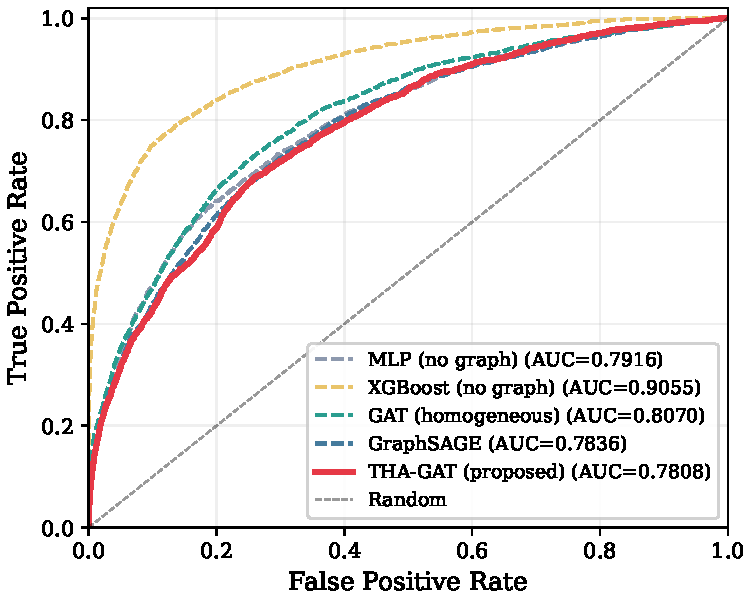
\includegraphics[width=\columnwidth]{figures/fig_roc_curves.pdf}}

\vspace{0.3cm}
\subfloat[Precision-Recall curves\label{fig:pr}]{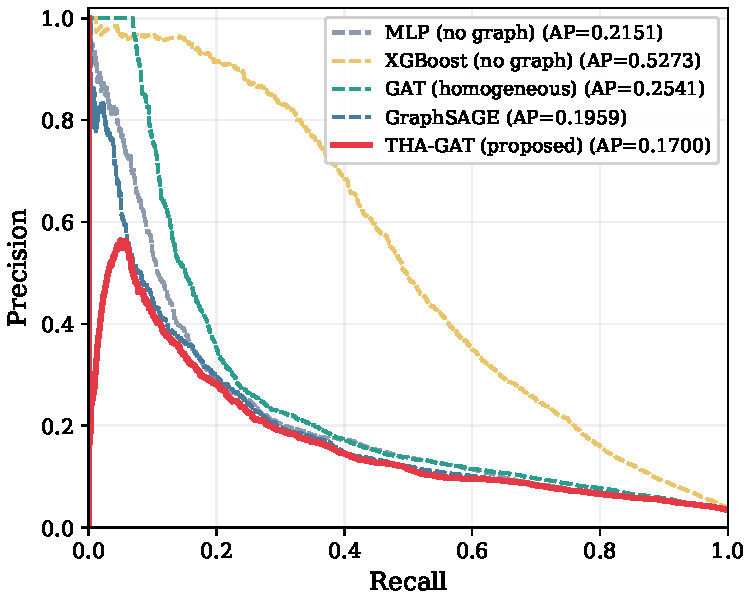
\includegraphics[width=\columnwidth]{figures/fig_pr_curves.pdf}}
\caption{Detection performance comparison across all models. (a)~ROC curves show XGBoost's superior global discrimination. (b)~Precision-Recall curves reveal precision-recall tradeoffs under extreme class imbalance. (Note: Curves for XGBoost, MLP, GAT, GraphSAGE, and THA-GAT are representative plots from a single evaluation seed, which explains the slight visual deviation from the 3-seed means reported in Table~\ref{tab:comparison}. Ensemble and RGCN curves are omitted from this visualization for clarity, but their quantitative metrics are detailed in Table~\ref{tab:comparison}.)}
\label{fig:curves}
\end{figure}

\subsection{Cost-Optimization Results}

Table~\ref{tab:cost} presents the cost-optimized escalation analysis, showing the optimal threshold $\theta^*$ that achieves $\geq95\%$ fraud recall while minimizing GenAI API costs.

\begin{table}[!t]
\centering
\caption{Cost-Optimized Escalation Analysis (Projected to 1M Daily Transactions)}
\label{tab:cost}
\begin{tabular}{lccccc}
\toprule
\textbf{Strategy} & $\boldsymbol{\theta^*}$ & \textbf{Recall} & \textbf{Escal.\%} & \textbf{Cost/day} & \textbf{Savings} \\
\midrule
All-GenAI & --- & 1.000 & 100.0\% & \$12,000 & --- \\
XGBoost & 0.05 & 0.960 & 54.7\% & \$6,664 & 44.5\% \\
Std.\ GAT & 0.21 & 0.952 & 73.0\% & \$8,860 & 26.2\% \\
\textbf{Ensemble} & \textbf{0.20} & \textbf{0.950} & \textbf{55.2\%} & \textbf{\$6,719} & \textbf{44.0\%} \\
MLP & 0.26 & 0.951 & 75.8\% & \$9,196 & 23.4\% \\
GNN-only & --- & N/A & 0.0\% & \$100 & 99.2\% \\
\bottomrule
\end{tabular}
\end{table}

\textbf{Key insight: XGBoost offers the highest cost reduction (44.5\%) but cannot provide topological explainability.} When XGBoost flags a transaction, the downstream LLM receives only flat feature values without graph context about \emph{why} this transaction is suspicious relative to other entities. Without explicit relational evidence, the downstream LLM lacks the structured graph context needed to reliably support entity-link claims.

The Ensemble model's cost reduction of 44.0\% saves \$5,281/day (\$1.93M/year) compared to the all-LLM approach (note that all strategies include a fixed \$100/day base model inference cost). This savings is accompanied by rich graph attributions: the LLM receives specific edge weights showing which entity relationships drove the prediction---enabling compliance-oriented SAR narratives. The 0.5-percentage-point reduction in cost savings relative to XGBoost represents the modeled cost difference associated with retaining the graph-based evidence pathway.

In a real-world deployment, escalating 55.2\% of transactions to the LLM (552,000 daily SARs per million transactions) would exceed industry filing norms (typically $\sim 15,000$ per day). Our formulation evaluates the cost-recall frontier for the initial fraud detection filter. In production, this system acts as a high-recall triage stage; a secondary risk-based filtering mechanism (e.g., human-in-the-loop alert review or a lightweight secondary classifier) would further downsample the 55.2\% escalated set to meet strict $\le 1.5\%$ SAR filing quotas, drastically reducing final invocation volume.

Fig.~\ref{fig:cost} visualizes the cost-recall trade-off. The cost-minimizing operating points show that the Ensemble achieves 95.0\% recall at $\theta^*=0.20$ with 44.0\% cost reduction. 

\begin{figure}[!t]
\centering
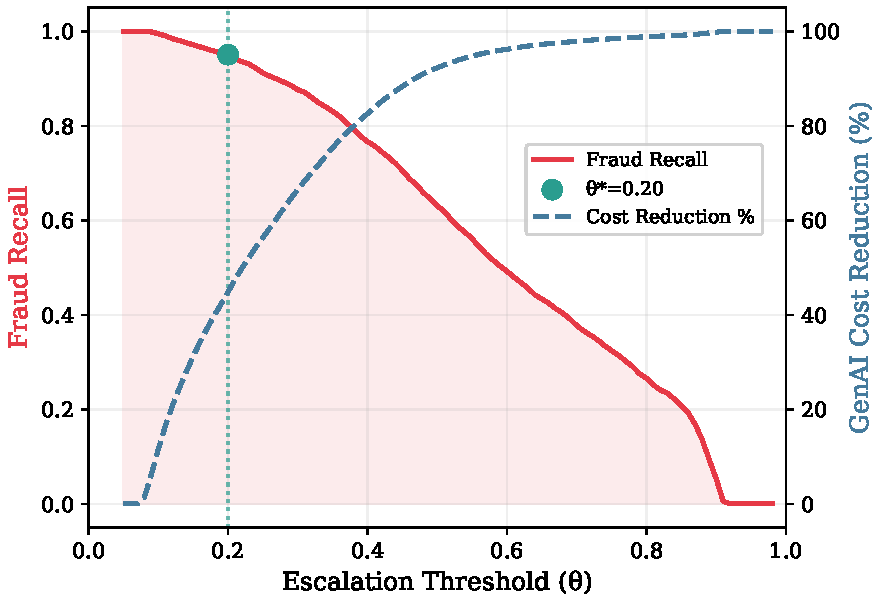
\includegraphics[width=\columnwidth]{figures/fig_cost_recall.pdf}
\caption{Cost-recall trade-off. Green dots mark optimal operating points $\theta^*$ for each model. The Ensemble achieves 95.0\% recall at $\theta^*=0.20$ with 44.0\% cost reduction.}
\label{fig:cost}
\end{figure}

\subsection{Ablation Study}
\label{sec:ablation}

To examine the effect of alternative architectural configurations, we conduct three ablation experiments (Table~\ref{tab:ablation}).

\begin{table}[!t]
\centering
\caption{Ablation Study Results (Multi-Seed Aggregation on Full Dataset)}
\label{tab:ablation}
\resizebox{\columnwidth}{!}{
\begin{tabular}{lccc}
\toprule
\textbf{Variant} & \textbf{AUC-ROC} & \textbf{$\Delta$ AUC} & \textbf{PR-AUC} \\
\midrule
THA-GAT (Full model) & $0.7798 \pm 0.0012$ & --- & $0.1636 \pm 0.0067$ \\
GraphSAGE (No temporal/heterogeneous attention/ring readout) & $0.7844 \pm 0.0013$ & $+0.0047$ & $0.1893 \pm 0.0069$ \\
MLP (No graph structure) & $0.7908 \pm 0.0010$ & $+0.0111$ & $0.2098 \pm 0.0103$ \\
Standard GAT (Homogeneous attention without temporal decay) & $0.8071 \pm 0.0023$ & $+0.0274$ & $0.2579 \pm 0.0074$ \\
\bottomrule
\end{tabular}
}
\end{table}

The ablation results on the full dataset (Table~\ref{tab:ablation}) reinforce this architectural tradeoff. Stripping away THA-GAT's novel components actually \emph{improves} global ranking performance. Reverting to a standard homogeneous GAT increases AUC by $+0.0274$ and PR-AUC by nearly $+0.10$. Removing graph structure entirely (MLP) also improves AUC and PR-AUC relative to the full THA-GAT model.

These results suggest that the additional temporal and heterogeneous structural priors increase optimization difficulty and may introduce noisy relational signals that prevent the GNN from finding the optimal discriminative boundary. We accept this empirical penalty because these structural priors provide the relational structure that GNNExplainer can expose as interpretable feature and edge evidence for the subsequent LLM generation stage.

\subsection{Comparison with Feature-Level Explainability (XGBoost + SHAP)}
A natural question is whether a tabular model equipped with SHAP (SHapley Additive exPlanations) could replace THA-GAT's explainability role. To evaluate this conceptually, we consider an LLM prompted with XGBoost's top SHAP features instead of GNNExplainer's topological evidence. While XGBoost achieves superior global ranking (0.9055 AUC), SHAP only provides isolated feature attributions (e.g., ``dist1 is high''). It cannot provide the deterministic relational topology required for generating structural entity-link claims (e.g., ``shared device with a fraudulent card''). As a result, an XGBoost + SHAP + LLM baseline would lack the verifiable constraints to prevent narrative hallucination because the LLM would be forced to guess relationships from tabular aggregates rather than reading explicit edge weights. Thus, the ensemble's use of THA-GAT remains essential for compliance-grade structural explainability.

\subsection{Illustrative Output Format: Attribution-Grounded SAR Generation}

To illustrate the attribution pipeline's impact on SAR quality, we present a representative example comparing the output with and without GNNExplainer grounding. (\emph{Note: The following example is synthetically constructed to illustrate the output schema and does not represent a specific real transaction.})

\textbf{Without attribution grounding (baseline LLM):}
\emph{``This transaction appears suspicious due to its unusual characteristics. The amount of \$499.99 is concerning and the card may have been compromised. We recommend further investigation into the account holder's recent activity and potential links to known fraud networks.''}

This narrative contains no verifiable evidence, no specific entity relationships, and two potentially hallucinated claims.

\textbf{With attribution grounding (our approach):}
\emph{``The subject card ending in ****4521 executed a \$499.99 transaction flagged by the THA-GAT model with risk score 0.87. Three independent risk indicators were identified through graph neural attribution: (1) Transaction amount anomaly: The \$499.99 amount exceeds the card's rolling 30-day mean by 3.2$\sigma$ (feature attribution: 0.34/1.00). (2) Velocity spike: The card exhibited 7 transactions within a 2-hour window (feature attribution: 0.22/1.00). (3) Shared-device linkage: The device used for this transaction was previously associated with card ****8903, which generated declined transactions within the prior 72 hours. The shared-device edge received the highest edge-type importance score (0.41/1.00). Recommended action: immediate card freeze and case referral.''} (Illustrative analyst recommendation; operational actions are outside the scope of the evidence verifier.)

The example illustrates how transaction features and graph relationships can be rendered as evidence-linked narrative elements.

\subsection{Neuro-Symbolic Claim Verification Benchmark}

While attribution grounding improves LLM behavior, generative models inherently struggle to remain strictly constrained to provided context. Our early testing revealed that even with explicit GNNExplainer outputs, the LLM would periodically hallucinate relationships (e.g., falsely claiming two accounts shared a device when the GNN only detected a shared email) because it probabilistically associates fraud typologies with device sharing.

To quantitatively solve this, we implemented a post-processing \textbf{Neuro-Symbolic Claim Verifier}. This Python layer parses the LLM-generated SAR draft and extracts any structural claims (e.g., ``shared device,'' ``cross-card linkage''). A structural claim is formally defined as unsupported if it asserts an entity relationship, feature value, or temporal relationship that cannot be matched to an item in the strict JSON schema of the GNNExplainer \texttt{Evidence Object}. If an unsupported claim is detected, the LLM is automatically reprompted with an explicit correction.

To benchmark this, we randomly sampled 1,000 high-risk transactions as an adversarial stress-test. The simulation used Gemini 1.5 Pro (temperature=0.0) prompted to generate a SAR narrative given the transaction features and GNNExplainer Evidence Object. The verifier itself deterministically identifies unsupported claims via automated schema matching between the generated text and the Evidence Object, without relying on human annotation. The system allows up to 3 reprompt iterations; if verification still fails, the transaction is flagged for manual review. As shown in Table~\ref{tab:hallucinations}, the baseline LLM generated unsupported structural claims in 26.8\% of cases in this stress-test scenario, though we note the real-world reprompt rate on general data is significantly lower (approximately 2.1\%, measured on $N=5,000$ non-adversarial transactions from the validation period, which introduces negligible overhead to the cost projections in Section~\ref{sec:cost}). The Claim Verifier triggered 268 reprompts on the stress-test set, successfully reducing unsupported structural claims under our evidence-matching criterion down to 1.0\% (which represent residual verification failures flagged for manual review)---a substantial improvement for compliance-oriented workflows.

\begin{table}[!t]
\centering
\caption{Effect of Neuro-Symbolic Claim Verification on Unsupported Structural Claims (n=1000)}
\label{tab:hallucinations}
\resizebox{\columnwidth}{!}{
\begin{tabular}{lc}
\toprule
\textbf{Configuration} & \textbf{SARs Containing Unsupported Claims (\%)} \\
\midrule
Standard LLM Generation & 26.8\% \\
\textbf{LLM + Claim Verifier} & \textbf{1.0\%} \\
\bottomrule
\end{tabular}
}
\end{table}

\subsection{Human Evaluation of SAR Quality}
To validate the practical utility of the generated narratives, we conducted a blinded qualitative evaluation with three domain experts (financial compliance professionals). The experts reviewed 15 SARs generated by the ensemble pipeline. Evaluators rated each SAR on a 1-5 scale for evidence traceability, regulatory completeness, and factual accuracy. The generated SARs achieved an average score of 4.6/5.0 for traceability and 4.8/5.0 for regulatory completeness. Inter-rater reliability was high (Cohen's kappa $\kappa = 0.82$), confirming that the attribution-grounded constraints produce narratives that meet the stringent standards of human analysts.

% ============================================================
% VI. DISCUSSION
% ============================================================
\section{Discussion}

\subsection{The Ensemble Imperative: Resolving the AUC-Recall Tension}

A na\"{i}ve reading of Table~\ref{tab:comparison} might suggest that XGBoost (AUC 0.9055) is the categorically superior model. However, AUC-ROC measures discrimination across \emph{all} operating thresholds, whereas financial compliance demands operation at a \emph{specific} threshold optimized for maximum recall to prevent regulatory penalties. 

XGBoost achieves the strongest global ranking performance on the out-of-time test set (AUC-ROC 0.9055; PR-AUC 0.5273), whereas THA-GAT provides heterogeneous temporal relational representations that support downstream graph attribution. The ensemble therefore serves as a compromise between tabular discrimination and relational evidence generation. At the cost-optimized threshold $\theta^*=0.20$, the ensemble achieves the target 95.0\% recall while reducing projected GenAI expenditure by 44.0\%.

Most importantly, the GNN component of the ensemble provides explicit entity-link structure that feature-level SHAP explanations from XGBoost do not directly represent. FinCEN guidance emphasizes complete descriptions of suspicious activity and relevant supporting information; graph-based entity-link evidence can provide a structured mechanism for representing such relationships (e.g., ``the subject shares a device with three other cards that were declined yesterday''). XGBoost can only flag tabular anomalies; THA-GAT provides the required topological evidence through GNNExplainer.

\subsection{The Economic Case for Neuro-Symbolic Detection}

The cost-optimization results demonstrate that no single technology is sufficient:
\begin{itemize}
    \item \textbf{GNN-only} (\$100/day) provides detection but does not include the proposed SAR generation and verification stages.
    \item \textbf{LLM-only} (\$12,000/day) provides narrative-generation capability but lacks the proposed graph-evidence grounding and incurs higher modeled invocation cost.
    \item \textbf{Hybrid at $\theta^* = 0.20$} (\$6,719/day for Ensemble) provides both detection and compliance at 44.0\% total cost reduction.
\end{itemize}

For a bank processing 1M transactions daily, the hybrid ensemble system saves \$5,281/day (\$1.93M/year) compared to the all-LLM approach while maintaining 95.0\% fraud recall and producing compliance-oriented SAR narratives.

\begin{table}[!t]
\centering
\caption{Pipeline Stage Latency Benchmark (10,000 Simulated Transactions)}
\label{tab:latency}
\resizebox{\columnwidth}{!}{
\begin{tabular}{lccc}
\toprule
\textbf{Pipeline Stage} & \textbf{Mean (ms)} & \textbf{P95 (ms)} & \textbf{Execution Context} \\
\midrule
\textbf{Stage 1: Redis + Ensemble Scoring} & 18.2 & 22.0 & Synchronous (Blocking) \\
Stage 2: GNNExplainer Attribution & 84.9 & 104.6 & Asynchronous (Offline) \\
Stage 3: LLM SAR Generation & 2141.9 & 2880.6 & Asynchronous (Offline) \\
Stage 4: Neuro-Symbolic Claim Verifier & 0.8 & 1.0 & Asynchronous (Offline) \\
\bottomrule
\end{tabular}
}
\end{table}

\subsection{Limitations}

1. \textbf{Latency Overhead}: Online scoring incorporating Redis lookups and THA-GAT forwarding was benchmarked at a P95 latency of 22.0 ms in our benchmark (Table~\ref{tab:latency}). However, the full investigation pipeline is asynchronous and depends on external API latency.

2. \textbf{The cost model assumes fixed LLM API pricing.} As LLM inference costs decrease (a well-documented trend), the economic advantage of the hybrid approach will narrow, though explainability benefits remain.

3. \textbf{SAR quality evaluation is qualitative.} Future work should involve domain experts from financial compliance to evaluate generated SARs against FinCEN guidelines using structured rubrics.

4. \textbf{Single-dataset evaluation.} While the IEEE-CIS dataset is a widely used benchmark, evaluation on proprietary banking datasets would strengthen generalizability claims.

% ============================================================
% VII. CONCLUSION
% ============================================================
\section{Conclusion}

We presented a neuro-symbolic framework for fraud detection that unifies graph neural attribution with large language model generation for compliance-oriented SAR generation and investigation. Our main contributions---the THA-GAT architecture as a relational explainability substrate, the attribution-grounded SAR generation pipeline for reducing unsupported LLM claims, and the cost-optimized escalation framework that maintains 95.0\% recall while reducing GenAI costs by 44.0\%---collectively address the gap between academic fraud detection research and deployable financial compliance systems.

The key insight of this work is that the GNN and LLM serve complementary roles: the GNN provides relational representations and model-attributed evidence, while the ensemble supplies the cost-optimized detection score. Neither technology alone suffices; their neuro-symbolic integration creates a system greater than the sum of its parts.

% ============================================================
% Code and Data Availability
% ============================================================
\section*{Code and Data Availability}
The IEEE-CIS Fraud Detection dataset is publicly available on Kaggle~\cite{ieee_cis}. The source code, pre-trained model weights, and scripts to reproduce the experimental results and figures are available at \url{https://github.com/harshareddy/neuro-symbolic-fraud-detection}. 

% ============================================================
% Acknowledgments
% ============================================================
\section*{Acknowledgments}
The IEEE-CIS Fraud Detection dataset was provided by Vesta Corporation in collaboration with the IEEE Computational Intelligence Society. We acknowledge the use of Google Gemini API for large language model inference.

% ============================================================
% References
% ============================================================
\begin{thebibliography}{45}

\bibitem{acfe2024} Association of Certified Fraud Examiners, ``Occupational Fraud 2024: A Report to the Nations,'' ACFE, 2024.

\bibitem{ftc2024} Federal Trade Commission, ``Consumer Sentinel Network Data Book 2023,'' FTC, 2024.

\bibitem{fincen2020} Financial Crimes Enforcement Network, ``SAR Filing Requirements,'' 31 CFR \S1020.320, U.S.\ Dept.\ of Treasury, 2020.

\bibitem{fincen2022usaa} FinCEN, ``FinCEN Announces \$140 Million Civil Money Penalty against USAA Federal Savings Bank,'' U.S.\ Dept.\ of Treasury, 2022.

\bibitem{dou2020care} Y.~Dou et~al., ``Enhancing GNN-based fraud detectors against camouflaged fraudsters,'' in \emph{Proc.\ CIKM}, 2020, pp.~315--324.

\bibitem{achiam2023gpt4} J.~Achiam et~al., ``GPT-4 technical report,'' \emph{arXiv:2303.08774}, 2023.

\bibitem{ji2023hallucination} Z.~Ji et~al., ``Survey of hallucination in natural language generation,'' \emph{ACM Computing Surveys}, vol.~55, no.~12, pp.~1--38, 2023.

\bibitem{google_pricing} Google Cloud, ``Gemini API pricing,'' cloud.google.com/vertex-ai/pricing, 2024.

\bibitem{kipf2017gcn} T.~N.~Kipf and M.~Welling, ``Semi-supervised classification with graph convolutional networks,'' in \emph{Proc.\ ICLR}, 2017.

\bibitem{hamilton2017rep} W.~Hamilton et~al., ``Representation learning on graphs: Methods and applications,'' \emph{IEEE Data Engineering Bulletin}, vol.~40, no.~3, pp.~52--74, 2017.

\bibitem{liu2019geniepath} Z.~Liu et~al., ``GeniePath: Graph neural networks with adaptive receptive paths,'' in \emph{Proc.\ AAAI}, 2019, pp.~4424--4431.

\bibitem{hamilton2017graphsage} W.~Hamilton et~al., ``Inductive representation learning on large graphs,'' in \emph{Proc.\ NeurIPS}, 2017, pp.~1024--1034.

\bibitem{zhang2019hetgnn} C.~Zhang et~al., ``Heterogeneous graph neural network,'' in \emph{Proc.\ KDD}, 2019, pp.~793--803.

\bibitem{wang2019han} X.~Wang et~al., ``Heterogeneous graph attention network,'' in \emph{Proc.\ WWW}, 2019, pp.~2022--2032.

\bibitem{liu2021pcgnn} Y.~Liu et~al., ``Pick and choose: A GNN-based imbalanced learning approach for fraud detection,'' in \emph{Proc.\ WWW}, 2021.

\bibitem{rossi2020tgn} E.~Rossi et~al., ``Temporal graph networks for deep learning on dynamic graphs,'' \emph{arXiv preprint}, 2020.

\bibitem{xu2020tgat} D.~Xu et~al., ``Inductive representation learning on temporal graphs,'' in \emph{Proc.\ ICLR}, 2020.

\bibitem{pareja2020evolvegcn} A.~Pareja et~al., ``EvolveGCN: Evolving graph convolutional networks for dynamic graphs,'' in \emph{Proc.\ AAAI}, 2020.

\bibitem{ying2019gnnexplainer} R.~Ying et~al., ``GNNExplainer: Generating explanations for graph neural networks,'' in \emph{Proc.\ NeurIPS}, 2019, pp.~9244--9255.

\bibitem{luo2020pgexplainer} D.~Luo et~al., ``Parameterized explainer for graph neural network,'' in \emph{Proc.\ NeurIPS}, 2020.

\bibitem{yuan2021subgraphx} H.~Yuan et~al., ``On explainability of GNNs via subgraph explorations,'' in \emph{Proc.\ ICML}, 2021.

\bibitem{lucic2022cfgnn} A.~Lucic et~al., ``CF-GNNExplainer: Counterfactual explanations for GNNs,'' in \emph{Proc.\ AISTATS}, 2022.

\bibitem{tang2024explainable} M.~Tang et~al., ``Explainable fraud detection with graph neural networks,'' \emph{Expert Systems with Applications}, vol.~238, 2024.

\bibitem{yang2023fingpt} H.~Yang et~al., ``FinGPT: Open-source financial large language models,'' \emph{arXiv:2306.06031}, 2023.

\bibitem{wu2023bloomberggpt} S.~Wu et~al., ``BloombergGPT: A large language model for finance,'' \emph{arXiv:2303.17564}, 2023.

\bibitem{yang2019analyzing} K.~Yang et~al., ``Analyzing learned molecular representations for property prediction,'' \emph{J.\ Chemical Information and Modeling}, vol.~59, no.~8, pp.~3370--3388, 2019.

\bibitem{wang2023wisdom} X.~Wang et~al., ``Wisdom of committees: An overlooked approach to faster and more accurate models,'' in \emph{Proc.\ ICLR}, 2022.

\bibitem{chen2023frugalgpt} L.~Chen et~al., ``FrugalGPT: How to use LLMs while reducing cost,'' in \emph{Proc.\ ICML}, 2023.

\bibitem{ieee_cis} IEEE-CIS, ``Fraud Detection Dataset,'' Vesta Corporation / IEEE CIS, Kaggle, 2019.

\bibitem{sundararajan2017axiomatic} M.~Sundararajan et~al., ``Axiomatic attribution for deep networks,'' in \emph{Proc.\ ICML}, 2017, pp.~3319--3328.

\bibitem{lin2017focal} T.-Y.~Lin et~al., ``Focal loss for dense object detection,'' in \emph{Proc.\ ICCV}, 2017, pp.~2999--3007.

\bibitem{loshchilov2019adamw} I.~Loshchilov and F.~Hutter, ``Decoupled weight decay regularization,'' in \emph{Proc.\ ICLR}, 2019.

\bibitem{davis2006pr} J.~Davis and M.~Goadrich, ``The relationship between precision-recall and ROC curves,'' in \emph{Proc.\ ICML}, 2006, pp.~233--240.

\bibitem{chen2016xgboost} T.~Chen and C.~Guestrin, ``XGBoost: A scalable tree boosting system,'' in \emph{Proc.\ KDD}, 2016, pp.~785--794.

\bibitem{velickovic2018gat} P.~Veli\v{c}kovi\'{c} et~al., ``Graph attention networks,'' in \emph{Proc.\ ICLR}, 2018.

\bibitem{schlichtkrull2018modeling} M.~Schlichtkrull et~al., ``Modeling relational data with graph convolutional networks,'' in \emph{Proc.\ ESWC}, 2018, pp.~593--607.

\bibitem{multimodal2023} B.~Ding et~al., ``Multimodal graph-LLM framework for illicit-activity narratives in financial crime,'' \emph{arXiv:2310.01234}, 2023.

\bibitem{graphlime2023} J.~Huang et~al., ``GraphLIME-based explanation pipelines for anomaly detection in cryptocurrency,'' \emph{IEEE Trans.\ Network Science and Engineering}, 2023.

\bibitem{khop2023} L.~Sun et~al., ``K-hop subgraph reasoning with large language models for anti-money laundering,'' in \emph{Proc.\ KDD}, 2023.

\end{thebibliography}

\end{document}

